% report.tex - HPC 714 Report
% Uncomment the below line for the double spaced, review copy
% \documentclass[draftclsnofoot,onecolumn,conference,11pt]{IEEEtran}
% Uncomment the below line for the two column, final copy
\documentclass[conference,twocolumn,11pt]{IEEEtran}

% Load packages for the report
\usepackage{cite}
\usepackage{array}
\usepackage[caption=false,font=normalsize,labelfont=sf,textfont=sf]{subfig}
\usepackage{url}
\usepackage{color}
\newcommand{\kostasnote}[1]{\textcolor{blue}{\bf #1}}
\newcommand{\bennote}[1]{\textcolor{magenta}{\bf #1}}

% Graphics and figures configuration
\usepackage[pdftex]{graphicx}
% declare the path(s) where your graphic files are
\graphicspath{{./figures/}}
% and their extensions so you won't have to specify these with
% every instance of \includegraphics
\DeclareGraphicsExtensions{.pdf,.jpeg,.png}

% Math package configuration
\usepackage{amsmath}
\interdisplaylinepenalty=2500

% correct bad hyphenation here
\hyphenation{op-tical net-works semi-conduc-tor}


\begin{document}

% report title
\title{Actors for Distributed Dataflow}


% author names and affiliations
\author{
    \IEEEauthorblockN{Benjamin Bengfort}
    \IEEEauthorblockA{
    \textit{University of Maryland}\\
    Department of Computer Science\\
    Email: bengfort@cs.umd.edu\\
    }

    \and
    \IEEEauthorblockN{Allen Leis}
    \IEEEauthorblockA{\textit{University of Maryland}\\
    Department of Computer Science\\
    Email: aleis@umd.edu\\
    }

    \and
    \IEEEauthorblockN{Konstantinos Xirogiannopoulos}
    \IEEEauthorblockA{\textit{University of Maryland}\\
    Department of Computer Science\\
    Email: kostasx@cs.umd.edu\\
}}

% make the title area
\maketitle

% report abstract
\begin{abstract}
Recently, the Actor model of concurrency in distributed systems has regained popularity as cluster computing frameworks for large scale analytics have started becoming mainstream. In particular, the use of virtual actors has shown to provide automatic scaling and load balancing through virtual actor properties of perpetual existence, automatic instantiation, and locale transparency. This programming model appears to be ideal for data processing of streams of unbounded data sets, in a computing architecture of live, online processing of data. In this paper, we present the communication patterns of three such data processing applications using sets (or ``casts'') of Actors. We then model the communication behavior on a cluster using a simulation and show that the virtual actor model effectively encapsulates how a cluster should behave in response to variable volumes of data. We propose that this simulation strongly motivates future work towards generalizing virtual actor spaces for distributed computation.
\end{abstract}

\section{Introduction}

Sensors, web logs, and other timely data sources are increasingly being used for  real-time or on-demand applications that utilize machine learning models to quickly make predictions and adapt to changes reflected by the input data. Timely sources present a challenge as they are streams of unbounded, occasionally unordered data sets that must be computed upon in an online, real-time fashion rather than in batch. When these data sources are also variable (e.g. the volume of traffic can occasionally spike) then the underlying computing framework must be able to scale and balance the load or risk falling so far behind that the computation becomes meaningless. Scalability must also be \textit{effortless}, should ``just work'' by simply scaling out the cluster size, and be \textit{adaptive} so that the cluster can be fairly utilized by all available jobs. \bennote{accepted the above - nice!}

Because of the widespread adoption of distributed computing frameworks like MapReduce \cite{dean_mapreduce:_2008} and Spark \cite{zaharia_resilient_2012}, distributed computing in a cluster of (often virtualized) economic servers has become the default, general method of high performance data processing. These frameworks primarily abstract the details of parallelism and distributing computation away from the developer, and have allowed a wider community of programmers and scientists to take advantage of parallel algorithms and libraries. Machine learning in particular has come of age in this computing environment, and as a result there exist many high level libraries for fitting a wide array of models in parallel.

As a result, tools for dealing with \textit{streaming data} (unbounded, unordered, variable data sources) have mostly been contextualized similarly to parallel machine learning algorithms -- via descriptions of how data flows through the application. Tools like Spark Streaming \cite{zaharia_discretized_2012}, Storm \cite{toshniwal_storm_2014}, and Google DataFlow \cite{akidau_dataflow_2015} implement a \textit{data flow} programming model, where analysis is described as a directed graph whose nodes represent a single computation, and whose edges represent the transmission of input and output values. Describing computation this way is simple, adaptable, and when mapped to a distributed topology, scalable. However, this model does not allow nodes to \textit{communicate}, nor does it provide any flexibility in the computational topology for error handling, transactional guarantees, consistency, or persistence.

In response to this inflexibility of the data flow model, the \textit{actor model} \cite{hewitt_viewing_1977, agha_actors:_1985} has been re-emerging as an abstraction that allows for more versatility in communication between distributed processes while still being at a high enough level to abstract the details of communication within the cluster away from the programmer. Ironically, it is this model that underpins the more general data flow models \cite{gonzalez_asynchronous_2015}, perhaps due to the fact that these applications are implemented in the Scala programming language, which by default uses actors for concurrency \cite{haller_scala_2009,karmani_actor_2009}. Actors in this context are high level primitives that do not share state, making them ideal candidates for under-the-hood parallelism. However, a simple data structure alone is not enough for a distributed computing; there must also be an execution and job management context. Orleans \cite{bernstein_orleans:_2014} presents the idea of a ``virtual actor space'', analogous to virtual memory, such that actor activations (e.g. instances of a program) exist forever, are transparent to their locale, and are automatically instantiated and deactivated. Virtual actors therefore provide for automatic scaling and load balancing in the cluster, and we believe are a novel and suitable alternative to the data flow model in the context of online, streaming computation.

In this paper we investigate the potential of virtual actors for distributed computing on streaming data by simulating a computing cluster which implements a \textit{generalized virtual actor space}. A generalized virtual actor space replaces the programing model of virtual actors with a daemon service that runs in the background of all nodes in the cluster; allocating resources to a variety of actor programs in an on-demand fashion such that the resources can scale as variability of data streams changes, while balancing load across many ``always on'' computations that must share resources. We have simulated this framework by analyzing the communications patterns of three real-time applications: a traditional data flow, an online recommendation application, and a solar weather forecasting application. We then present an analysis of how the virtual actor model behaved in simulation on the cluster and show that this model is a suitable substitute for the data flow model.

The rest of this paper is organized as follows. In the first section we present the details of our distributed computing model using actors, and describe the generalized virtual actor space in detail. Following this, we describe the applications we analyzed, and how we built a communication model from each type of application. Finally, we describe our simulation methodology, present our results, and conclude with a discussion and future work.

\section{Distributed Computing Framework}

This section describes a distributed computing framework that utilizes \textit{virtual actors} and its implementation for handling always-on computations that deal with streaming data. This framework sets the stage for the analysis of applications and their communications patterns and informs the construction of the simulation.

\subsection{Actors for Concurrency}

Actors are a model for reasoning about concurrent computation which is inspired by the \textit{communication mechanisms} of a society of experts that engage in effective problem solving \cite{hewitt_viewing_1977}.  Like other distributed models, actors are event oriented where ``events'' are messages received from other actors, and therefore parallelism is demonstrated through the partial ordering of these events. At a higher level, actors can be seen as data or task parallel pieces of a larger overall computation which maintain their state (e.g. each actor is a SPMD program).

\bennote{I wasn't sure how to incorporate agha, though it needs to be added here.}

Actors embody the three fundamental properties of computation: (1) storage (state), (2) processing , and (3) communication. In the traditional model, actors provide a simple abstraction for units of computation that can be programmed. Using these three resources at their disposal, Actors provide an intuitive way to reason about concurrent computation; as they can be easily associated with the real world. Actors provide a simple, concise interface that contribute to the programmability of this model. Actors operate under three necessary and sufficient \textit{axioms}. In response to the receipt of a message, apart from \textit{altering its own state}, an actor can engage in one of three simple actions: They can (1) create a finite number of \textit{new} actors, (2) send a finite number of messages to other actors it has the addresses of, and (3) designate its behavior upon receiving the next message. According to the conceptual model, actors can process a single message at a time, but in practice, they can be implemented so that they can handle arbitrarily many messages at a time. %maybe connect this to the thing im saying below as to the fact that you can do different things under the hood shows the power of this abstraction.

We believe the power of the actor model lies in its simplicity, as well as its ability to concisely model the control flow of parallel computation as it naturally ``emerges'' out of the behavior of actor entities in response to the receipt of messages.

Actor model MIT dissertation \cite{hewitt_viewing_1977, agha_actors:_1985}


\subsection{Generalized Virtual Actor Space}

\begin{figure}[h]
    \centering
    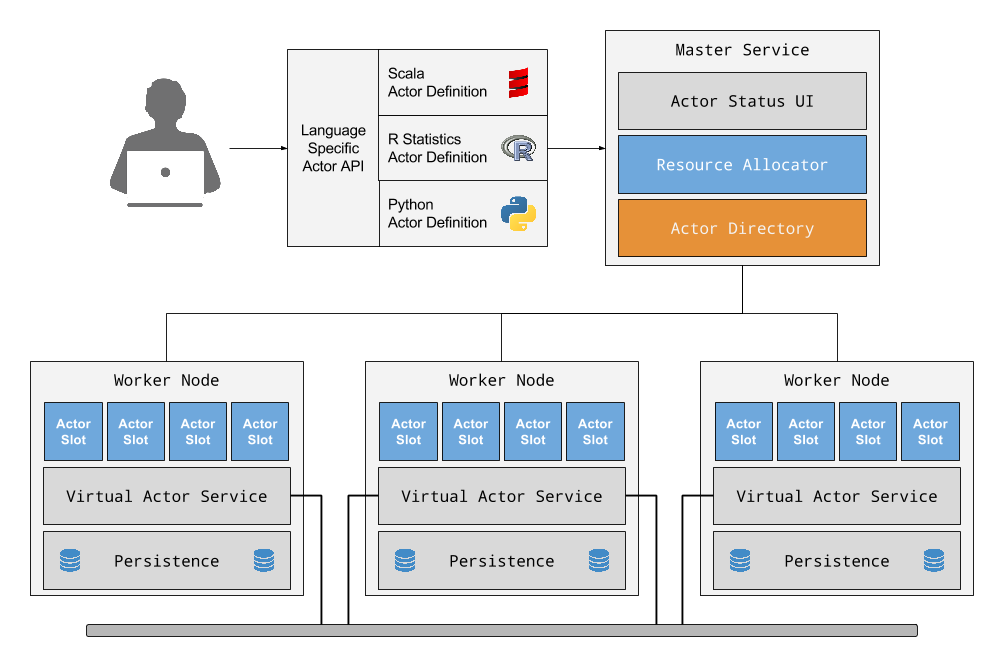
\includegraphics[width=0.45\textwidth]{architecture}
    \caption{The architecture for a generalized virtual actor framework.}
    \label{fig:architecture}
\end{figure}

The main source of inspiration for this work was the Orleans framework for building distributed applications. We believe Orleans' focus on \textit{programmability} and \textit{scalability} resonates with today's needs for ever-demanding large-scale distributed applications that need to be able to easily and continuously scale horizontally. The Orleans  framework defines a model based on a modernized variation of the actor model, known as a \textit{Virtual Actor Space}. In essence, a Virtual Actor Space consists of a set of virtual memory addresses, that can arbitrarily be used
- Orleans was inspired by and is a modern outlook on the traditional actor model.
- Basic idea: Virtual actors are logical entities that always exist. Actors have activations, and an activation can be spawned anywhere in the system. Actors are either stateful (only one activation at a time) or stateless (unboundedly scalable).
- Meant as a framework for easily and  intuitively programming distributed systems.

Orleans \cite{bernstein_orleans:_2014}



\section{Applications Analysis}

% This paragraph is pretty fundamental
In order to show that a generalized virtual actor framework is a distributed programming abstraction well suited to handling streaming data for online applications we must show two things: (a) that the model is a high level abstraction, friendly to programmers while also providing powerful concurrent guarantees and (b) that the model can be applied to real world problems in an efficient and robust manner. We have begun to show the former in the last section where we described how programs are built using the actor framework, though additional future work such as an Actor based API would go farther to proving this. In this section, we explore the latter by analyzing how three streaming applications would be adapted to the actor model.

Our initial exploration led us to a wide variety of applications to simulate, from traditional HPC scientific computing applications like Lulesh to social applications like proximity notification services. As we begun to inspect these programs in detail, we noticed that many of them shared similar characteristics in their \textit{communication patterns} -- a fundamental aspect of actor based programming and streaming data in particular. In this section, we have identified three applications that typify the communications patterns we discovered. We have included a traditional data flow application for real-time email analysis, a realtime recommendation analysis for an online store, and finally an application that uses an ensemble of machine learning to predict solar flare activity from magnetometer data.

In this section, we present a brief description of the application along with a definition of the \textit{cast} of actors required for computation (e.g. an object level identification of the streaming processes in the application). We conclude the section with our identified communication patterns, as these patterns were primarily what we simulated to show that an actor based framework can be applied to real applications.

\subsection{Email Analysis Data Flow}

The streaming data flow pattern was initially popularized by Twitter with the release of their open source Apache Storm project \cite{toshniwal_storm_2014}, which itself was followed by the Apache Heron project \cite{kulkarni_twitter_2015} as Twitter's real-time processing needs outpaced the low resource consumption of the Storm architecture. Both Storm and Heron allow the user to create a \textit{topology} via a domain specific language (DSL). Topologies are directed, acyclic graphs of spouts and bolts, where a spout is a streaming data source that generates tuples of data to be fed into the topology, and bolts actually perform the computation upon those tuples. Bolts can transform incoming data and forward the information to other bolts downstream in the topology.

\begin{figure}[!h]
    \centering
    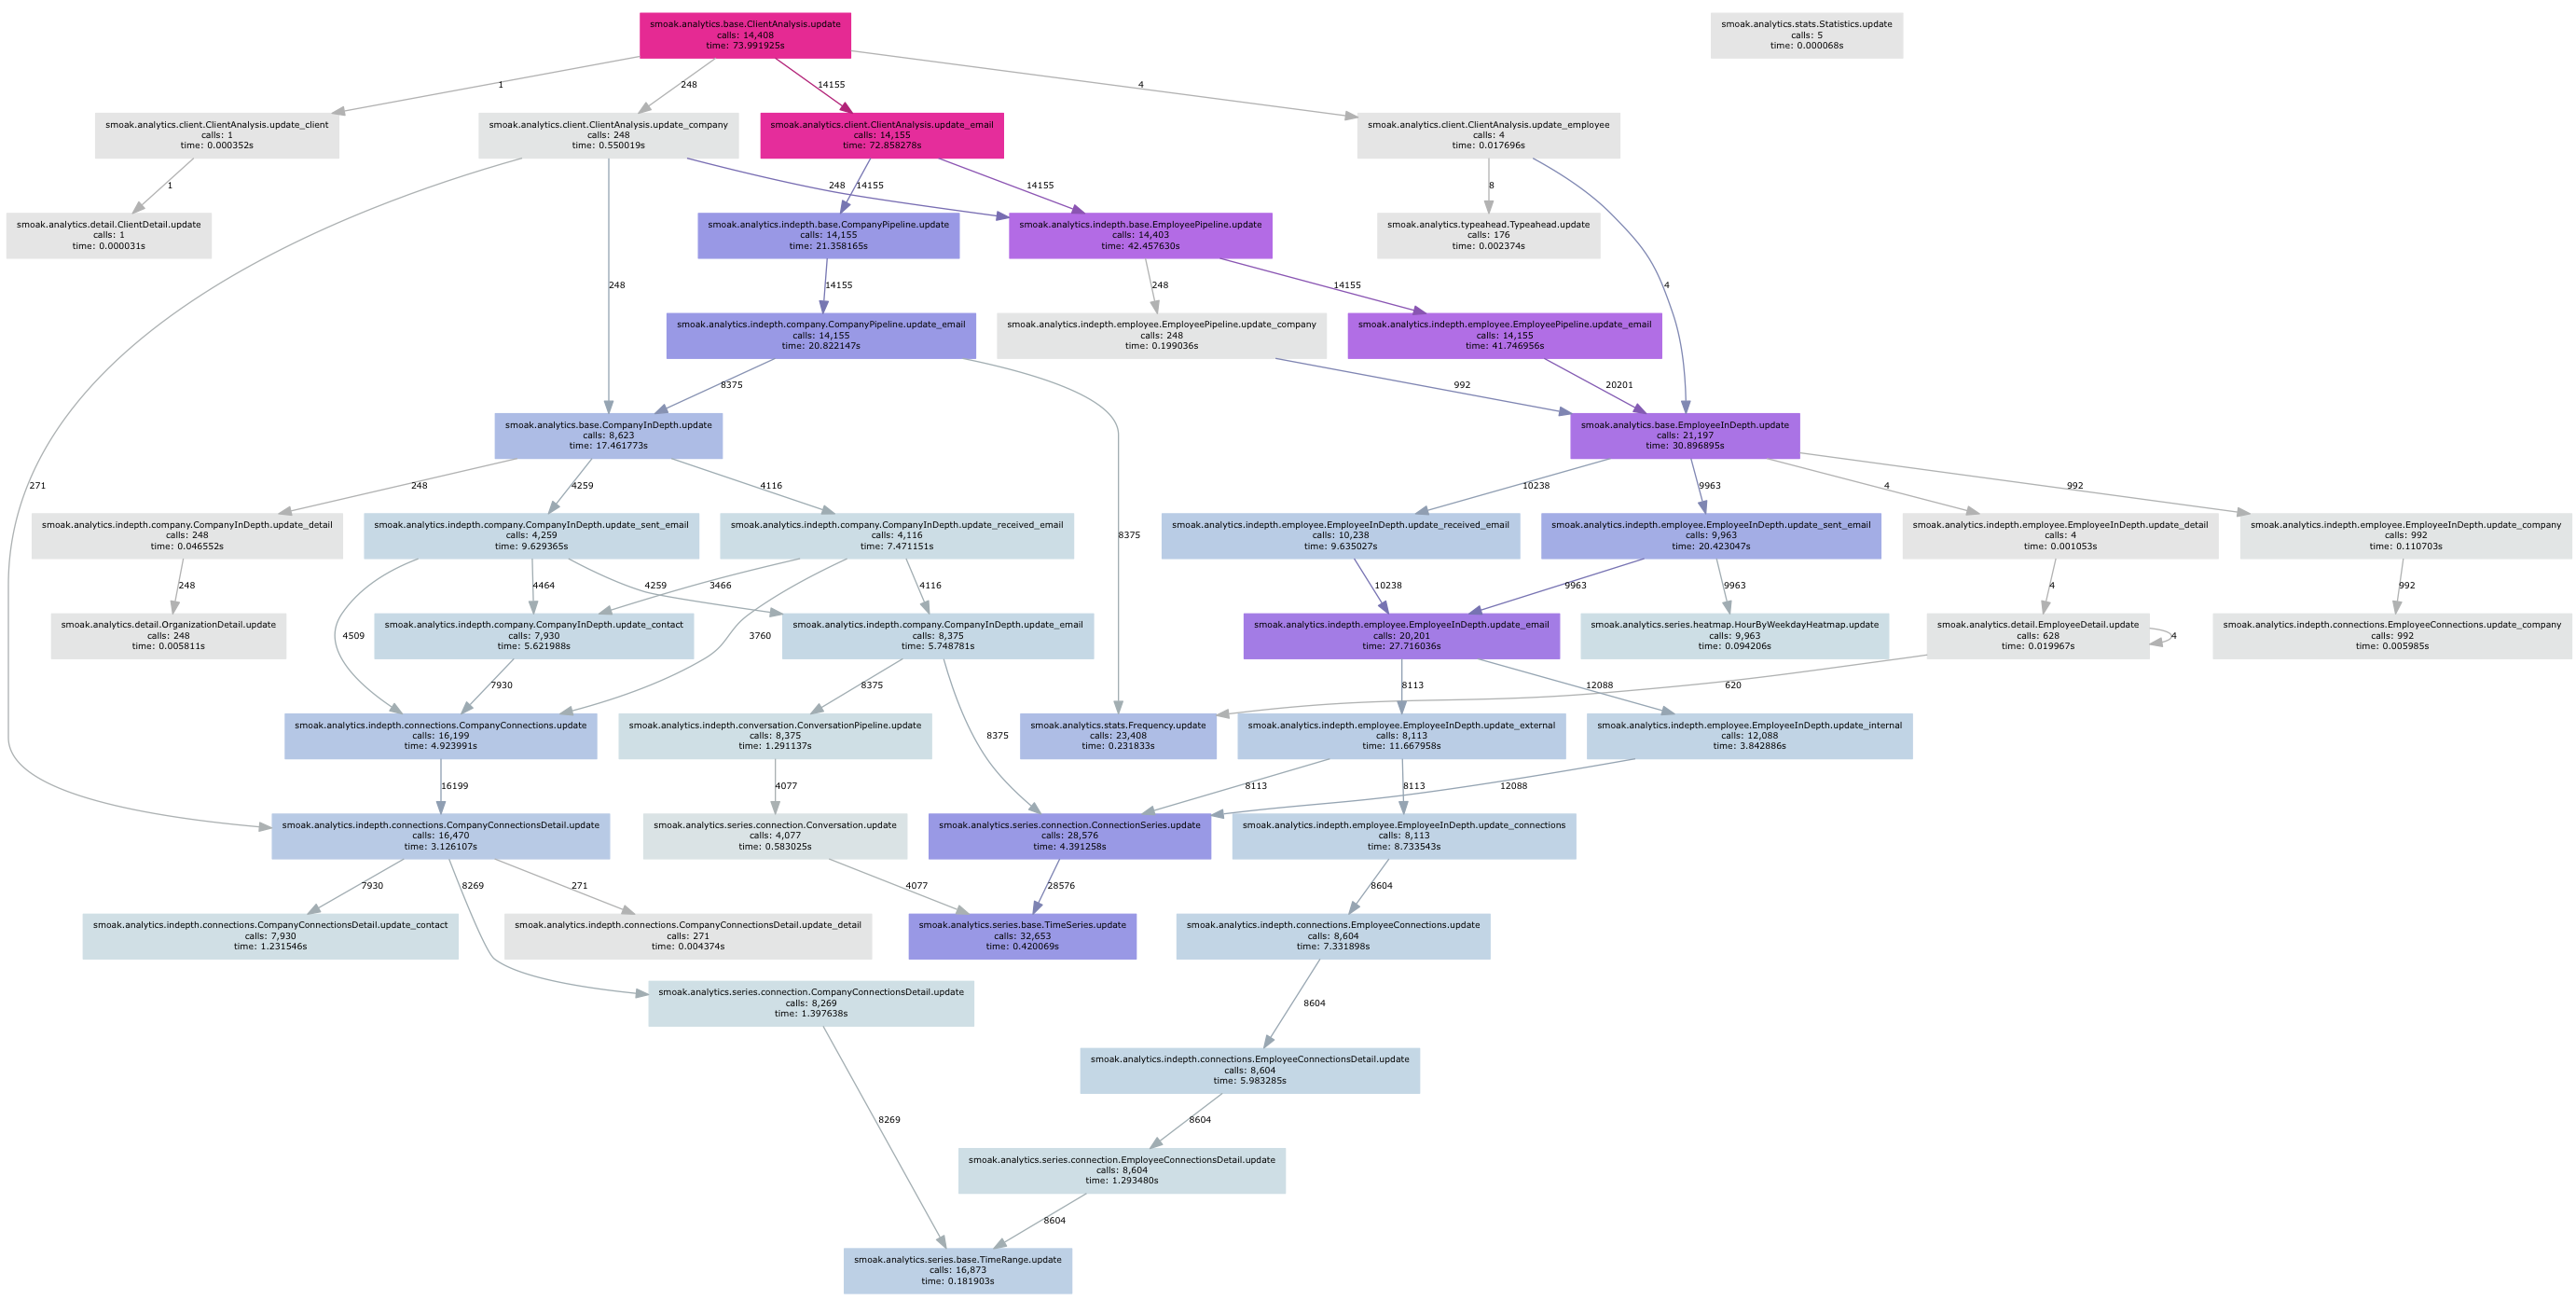
\includegraphics[width=0.45\textwidth]{dataflow_cast}
    \caption{The actor cast for a typical dataflow program.}
    \label{fig:dataflow_cast}
\end{figure}

Topologies in both Storm and Heron are essentially logical query plans that are then transformed into a physical query plan on a given system with a specific number of tasks. Shown in Figure \ref{fig:dataflow_cast} is the actor cast for a real implementation of a data flow for realtime email analysis. Topologies are often complex and conditionally executed based on the input data. Adding new tasks to a topology does not require modifying the entire data flow, but rather finding an insertion point where the input data matches the specification of the new tasks, and creating a new data flow. As such topologies themselves are often dynamic, responding to changes in the requirements of an application.

Because data flows provide data parallelism, concurrency is available in two places: different processes can process the same tuple in different points of the topology simultaneously and multiple process can implement a single bolt. Scalability in a data flow system involves the management of executors and communication in a topology, which is the fundamental difference between the Heron and Storm architectures. A primary concern in this type of architecture is that the message passing cost of processes distributed across the cluster can quickly overwhelm the benefit of parallelism, as processes do more waiting on messages than actual computation. However, when implemented correctly, this model is currently the defacto method of handling large scale streaming data, and thus an virtual actor framework must be able to implement similar computations as well if not better than the data flow standard.

\subsection{Online Recommendations}

The primary motivation for the use of the actor abstraction for distributed computing is to provide a programming model that allowed cyclic or direct inter-process communication between stateful nodes, something that the data flow model as proposed in the previous section cannot allow. This requirement is primarily related to online machine learning methods that utilize some form of optimization to fit a model, particularly linear models, clustering approaches, or training deep neural networks. Therefore, the second application we analyzed was that of a collaborative filtering system that provides real time recommendations for users as they browse an online store, viewing items or adding them to their cart.

\begin{figure}[!h]
    \centering
    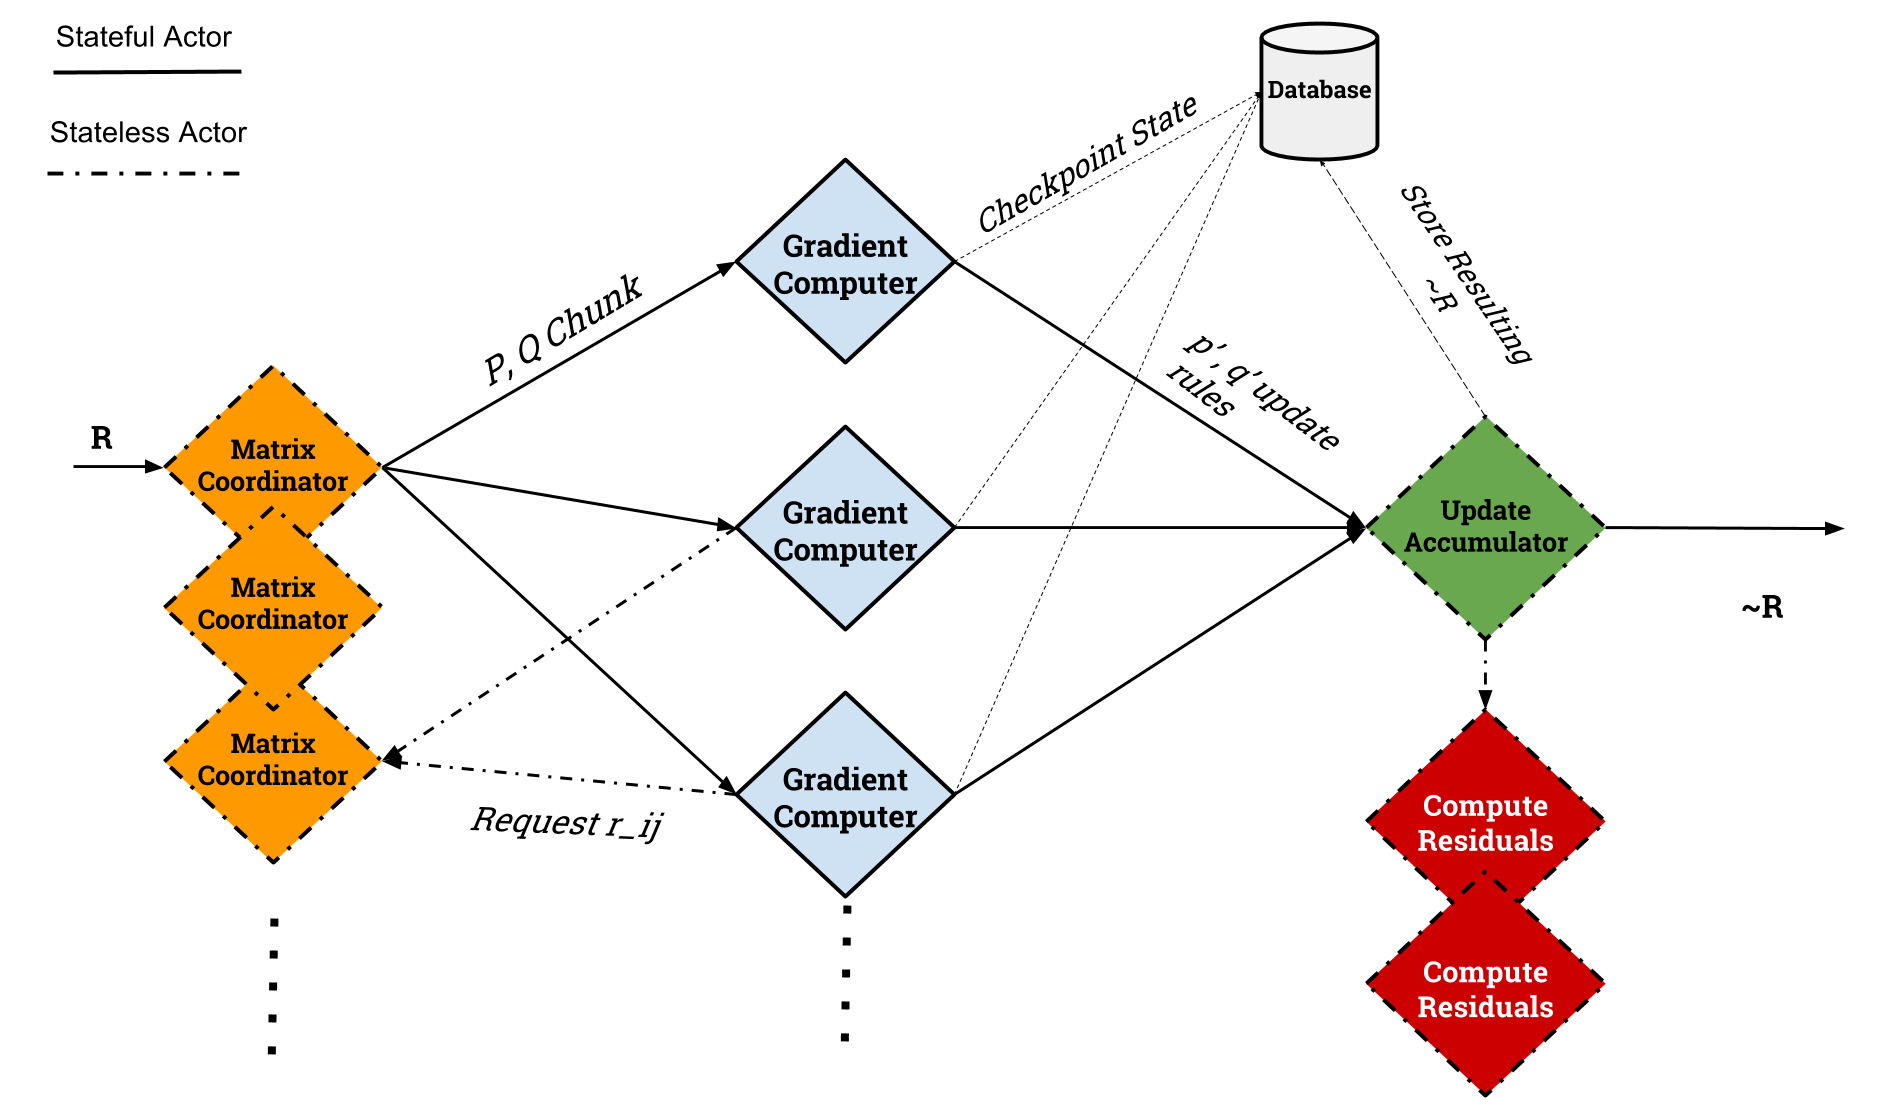
\includegraphics[width=0.45\textwidth]{nnmf_cast}
    \caption{The actor cast for implementing online recommendations with matrix factorization.}
    \label{fig:nnmf_cast}
\end{figure}

The most popular form of collaborative filtering for recommendations that are currently implemented are variations of the Netflix prize, which used a non-negative matrix factorization method with temporal dynamics \cite{koren_collaborative_2010}. Collaborative filtering involves the use of very sparse matrices, and sparse matrix factorization techniques for high performance computing is well studied \cite{gupta_highly_1997}. Currently the most popular algorithms used for parallel matrix factorization in recommenders are alternating least squares (ALS), which is implemented in the Spark MLLib as well as cyclic coordinated descent (CCD) \cite{yu_scalable_2012}.

Although both ALS and CCD could be implemented as actor casts, we have chosen to present an actor cast for distributed stochastic gradient descent (SGD) \cite{gemulla_large-scale_2011} as shown in Figure \ref{fig:nnmf_cast}. Distributed SGD is more generally applied and well understood. In this model, accumulators are required to buffer incoming streaming data while the model is being computed upon and multiple models can be computed simultaneously depending on data volume and partitioning schemes (for example by genre for a book store).

A set of actors decomposes the original, sparse matrix and begins the process of updating the divisors of the original matrix based on a learning rate and the derivative of the error curve. However, each gradient computer must also send horizontal information based on their computations to ensure that the dot product across the entire matrix is computed correctly, requiring interprocess communication. An accumulator aggregates the matrix tuples, which can then be fed to a parallel residuals computation. Although the details of this model are omitted for brevity, we want to primarily show that parallel and distributed algorithms can easily be implemented using an actor model, and in this case, with a cast of relatively few types of actors.

\subsection{Solar Flare Prediction}

The final application we analyzed is the most complex, and presents a significant challenge to both the traditional data flow model, as well as online machine learning. The inspiration for this analysis was a novel streaming data source, namely the 14 magnetic observatories across the northern hemisphere that monitor the earth's magnetic field for the USGS Geomagnetism Program \cite{love_usgs_2011}. Traditionally, the earth's magnetic field is modeled using scientific computing methods, however we believe that real-time Bayesian anomaly detection techniques \cite{hill_real-time_2007} might allow us to incoming predict solar weather based on currently observed anomalies.

\begin{figure}[!h]
    \centering
    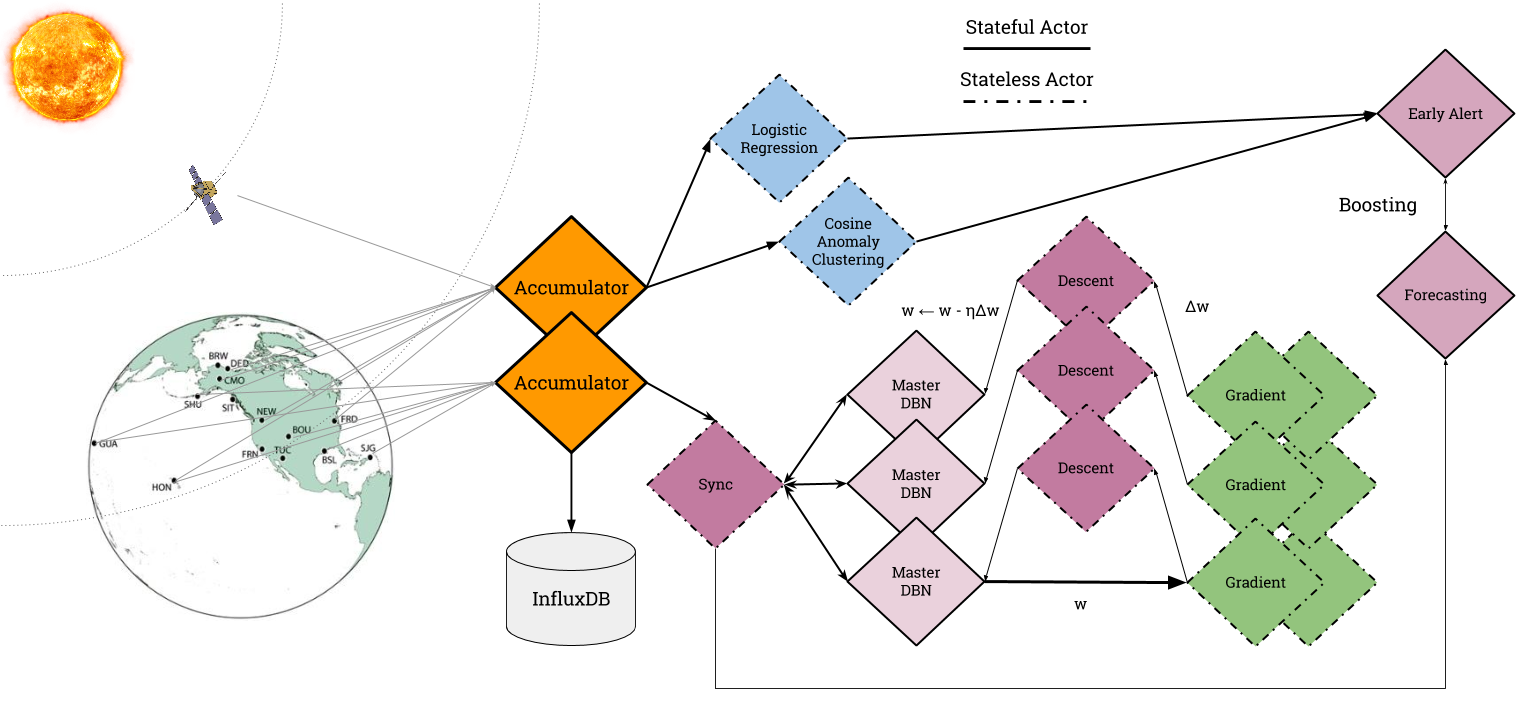
\includegraphics[width=0.45\textwidth]{solar_cast}
    \caption{The actor cast for a bagging approach to multiple machine learning models for solar flare prediction.}
    \label{fig:solar_cast}
\end{figure}

Bayesian approaches to solar flare prediction have been proposed in \cite{wheatland_bayesian_2004}, which notes that past activity of flares in a particular region of the Sun is a good indicator of future occurrences. Correlation of sunspot groups and flares using commonplace machine learning techniques was proposed in \cite{qahwaji_automatic_2007}. Furthermore, an analysis of short term sequential magnetosphere data (of the sun) was analyzed as features to supervised methods in \cite{yu_short-term_2009}, showing that three days worth of solar magnetosphere data was enough to predict flares; this approach was made more accurate using a multiresolution (e.g. boosting) approach that required less historical data to predict flares \cite{yu_short-term_2010}. None of these studies showed the relationship of predictors based on measuring the Earth's magnetosphere, however, we believe they are sufficient motivation for investigation into an actor cast implementation.

Although these observatories provide data in the form of vectors of the earth's magnetic field at a near constant rate, we propose that the on-demand scaling of a generalized virtual actor space is still useful in the context of an \textit{ensemble} of online machine learning methods. Here weaker, more compute efficient methods are used to detect anomalies at a broad granularity, while data is fed at a more stately rate to stronger, more compute-heavy mechanisms. However, when the weaker methods detect a potential anomaly at the higher granularity, the stronger methods are scaled to get a more precise outcome.

The actor cast shown in Figure \ref{fig:solar_cast} utilizes two weaker models (here logistic regression of timeseries information and cosine anomaly detection) to scale a Bayesian Deep Belief Network (DBN) on demand. The DBN is trained using yet another implementation of distributed optimization, here Downpour Stochastic Gradient Descent \cite{dean_large_2012}, which is specifically designed for large scale deep neural and deep belief networks.

\subsection{Communication Pattern Analysis}

\begin{figure*}[!t]
    \centering
    \subfloat[Email Dataflow]{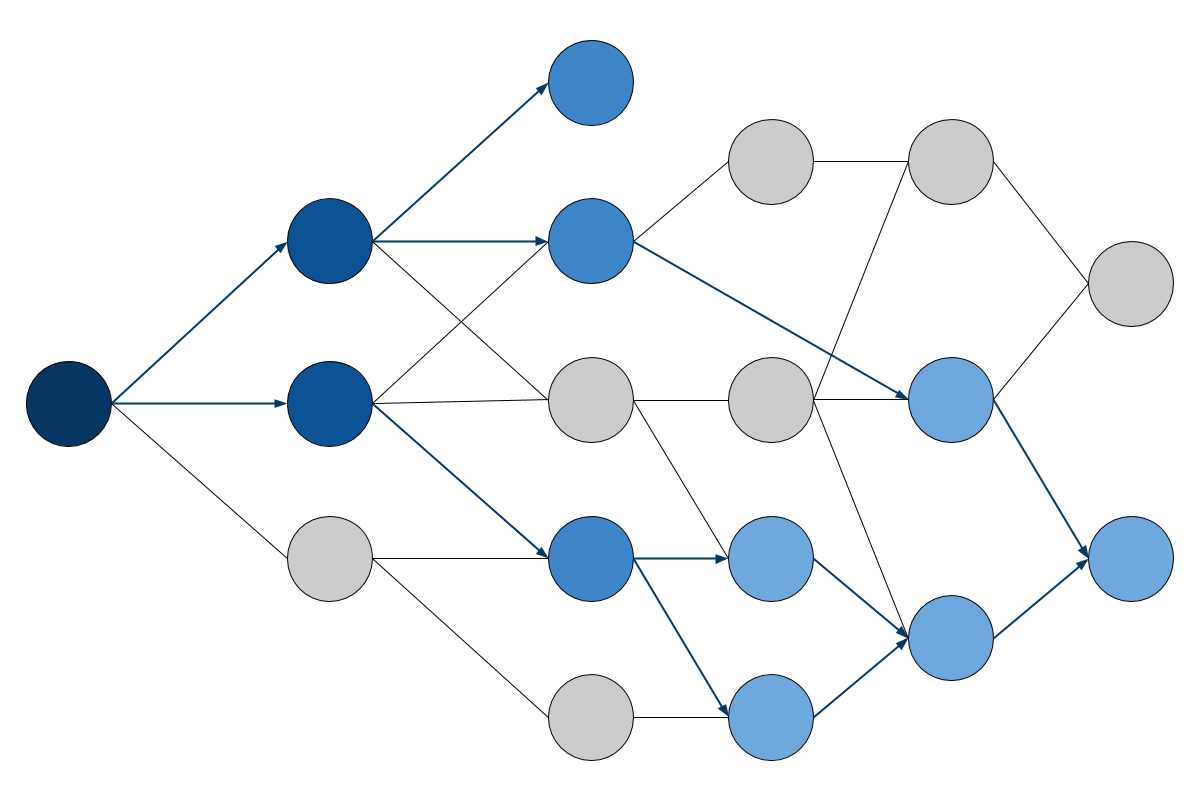
\includegraphics[width=0.3\textwidth]{dataflow_comms}
    \label{fig:dataflow_comms}}
    \hfil
    \subfloat[Online Recommendation]{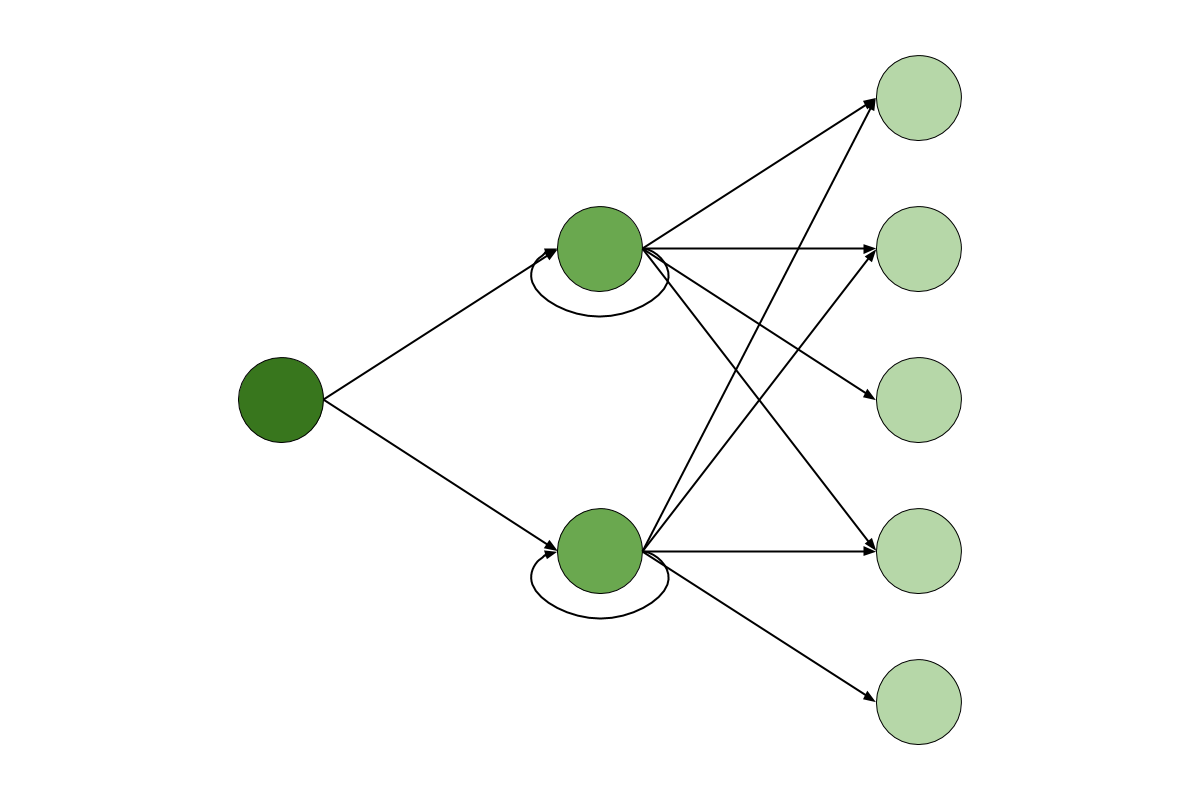
\includegraphics[width=0.3\textwidth]{nnmf_comms}
    \label{fig:nnmf_comms}}
    \hfil
    \subfloat[Solar Prediction]{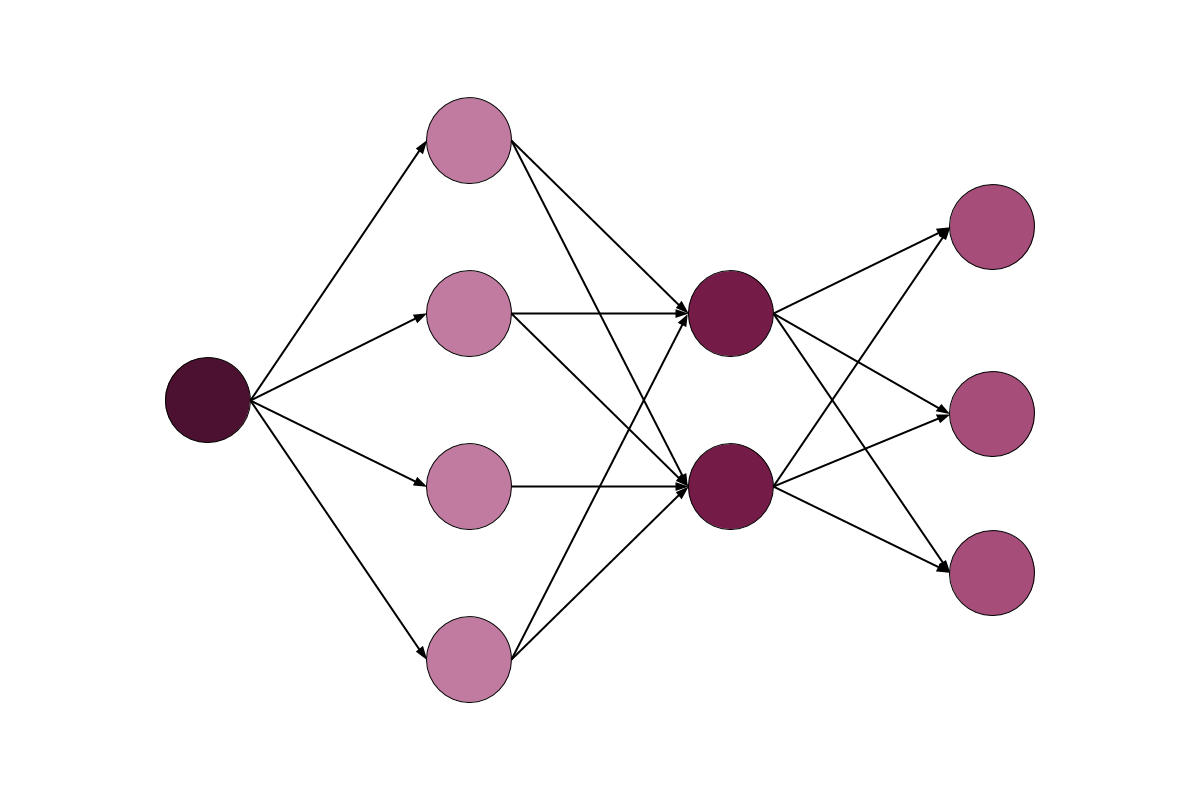
\includegraphics[width=0.3\textwidth]{solar_comms}
    \label{fig:solar_comms}}
    \caption{The corresponding communications patterns that we developed from these applications included branching, partial communication, iterative, front-loaded communication, and multiple-channel, full communication.}
    \label{fig:communications_patterns}
\end{figure*}

As we analyzed the above applications we began to notice that they broadly defined a more general communication pattern. Actors are inherently about communication, therefore our approach became to first model the application as an actor cast, then abstract each cast into a more general communication pattern. We then used these more general communications patterns as a guide to simulate the implementation of these applications. By simulating the general communication pattern, we hope to show that we can cover a wider array of applications and show how generalized virtual actor space load balances and scales in the face of variable data streams.

Figure \ref{fig:communications_patterns} shows the corresponding communications patterns we developed from each application. The email dataflow application (a) shows a communication pattern that is unidirectional and that includes branching, partial communication. In this application a message is replicated across the cluster, usually less times than there are actors. The online recommender (b) however, shows a communication model that is front loaded, and iterative; here more messages are generated during processing than those that are incoming. These messages are then passed downstream to finalizing actors where there is more balance. Finally, the solar prediction application (c) instead reflects a multi-channel, full communication approach; where data is buffered at the front (e.g. the weaker models) then boosted through the stronger models (representing a bottleneck) before being output at the end.

While these simplifications necessarily gloss over the computational requirements of an actor cast implementation of these applications, we believe that a focus on the communication patterns of actors represents the weakest point in a generalized virtual actor space. Techniques like speculative execution and heartbeat monitoring of processes allow for fault tolerance inside of communication, however the primary scaling and load balancing techniques are based solely on message load and throughput. In the next section we will discuss how we implemented our simulation of actor communication.

\section{Simulation Methodology}

Simpy \cite{matloff_introduction_2008}

\begin{figure}[!h]
    \centering
    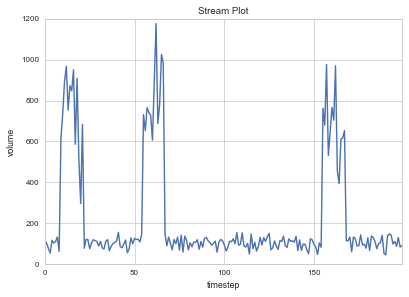
\includegraphics[width=0.45\textwidth]{streaming}
    \caption{Variable streaming data source with spikes of high activity, and longer periods of normal activity.}
    \label{fig:streaming}
\end{figure}

Our streaming data simulation is shown in Figure \ref{fig:streaming}.

% TODO: Cluster framework and representation
% TODO: Parameters for the simulation (streaming is already above)
% TODO: Discuss evaluation metric, utilization

\section{Discussion}

% TODO: Discuss what we learned
% TODO: Future work, etc.
Creating this simulation was a great idea...
Allowed for reasoning about the behaviour of such a system in different workloads, communication patterns, and hardware setup configurations.

The results yielded by the simulation appear to be ...
Our goals overlooking future work are tri-fold. We are interested in continuing to potentially add complexity to the simulation, which will allow for even more precise results. We believe another fundamental piece of this is also focusing on providing an easy to use API that will allow for as intuitive as possible programmability and adaptability of a framework like this into a cluster. Finally, once we will begin building a prototype of the system and start using it.  We believe that the system building process will spawn new and exciting problems in this space that will motivate and guide our future research on these topics.

If the number of available actors doesn't exceed the expected traffic, then the queue will continue to grow; forcing a reconfiguration.

\section{Conclusion}
The conclusion goes here.

% This should be very brief

The Github repository with the code for our simulation can be found at \url{http://bit.ly/actors-simulation}.

% conference papers do not normally have an appendix


% use section* for acknowledgment
\section*{Acknowledgment}
We would like to thank Dr. Josh Rigler from USGS for discussing the magnetometer project with us, the available data sources and how it could be computed upon. We would also like to thank Dr. Michael Wiltberger from NCAR as well as Dr. Alan Susman from UMD who put us in touch with Dr. Rigler. Finally we'd like to thank Dr. Amol Deshpande for taking a look at our work and inspiring the initial actor model research.

% begin the references section.
\bibliographystyle{IEEEtran}
\bibliography{IEEEabrv,paper}



% that's all folks
\end{document}
